Im Nachfolgenden soll die Funktechnologie auf der diese Arbeit aufbaut beschrieben werden. LoRa (Long Range) bildet dabei die Pysikalische schicht wärend LoraWAN (Long Range Wide Area Network) die Netzwerkschicht übernimmt. Die genaue aufteilung kann der Abbildung \ref{fig:lora-lorawan-osi} entnommen werden.

\begin{figure}[H]
\centering
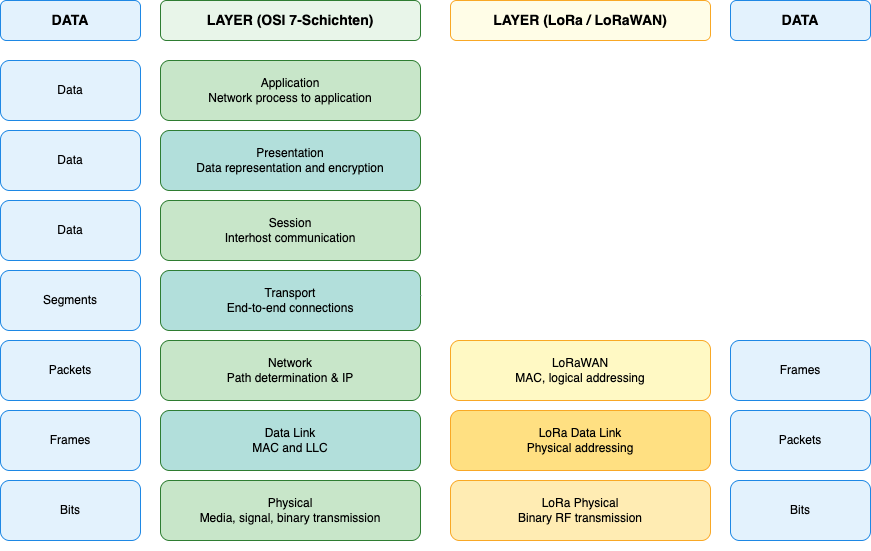
\includegraphics[scale=.4]{figures/diagrams/LoraWAN_OSI.png}
\caption{LoRa und LoRaWAN im OSI Schichtenmodell | Quelle: \ref{eckLoRaWANImDetail2019}}
\label{fig:lora-lorawan-osi}
\end{figure}

\subsubsection*{LoRa}
LoRa ist ein proprietäres und patentiertes drahtloses Übertragungsverfahren, das von der Semtech Corporation entwickelt wurde. Die Technologie arbeitet auf der physikalischen Schicht (Bitübertragungsschicht) und verwendet die Spread-Spectrum-Modulationstechnik \textit{Chirp Spread Spectrum} (CSS). CSS beinhaltet die Frequenzvariation eines Signals über die Zeit (Chirping). Ein „Upchirp“ ist eine Erhöhung der Frequenz von niedrig nach hoch, während ein „Downchirp“ eine Absenkung der Frequenz von hoch nach niedrig darstellt (siehe Abbildung \ref{fig:lora-chirp}). Diese Methode verteilt das Datensignal über ein breiteres Frequenzband, wodurch es robust gegenüber Rauschen und Interferenzen wird. 

\begin{figure}[H]
\centering
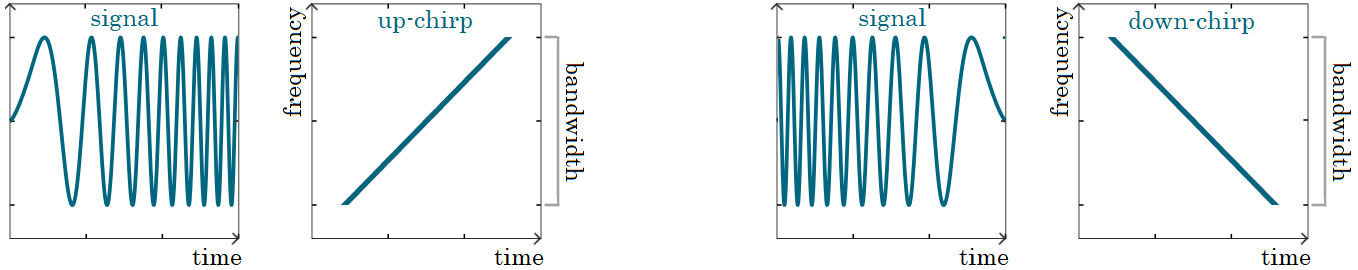
\includegraphics[scale=.4]{figures/asstes/lora-chirps.png}
\caption{LoRa Chirps | Quelle: \cite{tulkaLoRaSpreadingFactor}}
\label{fig:lora-chirp}
\end{figure}

Ein wesentlicher Vorteil von CSS gegenüber anderen Modulationstechniken, wie z.\,B. der in Abschnitt \ref{sec:drahtlosedatenübertragung} genannten FSK, ist die Fähigkeit, Signale selbst dann zu dekodieren, wenn sie unterhalb des Rauschpegels liegen. Dies wird durch die große Zeit-Bandbreite und die orthogonale Struktur der Chirp-Symbole ermöglicht.

\paragraph*{Spreading Factor} 
Der Spreading Factor (SF) beschreibt das Verhältnis zwischen der Chiprate und der Symbolrate. Wie aus Gleichung \ref{eq:spredigfactorbandwith} \cite[S.6]{rhode&schwarzCharacterizationLoRaDevices} ersichtlich, 
\begin{equation}
\label{eq:spredigfactorbandwith}
R_b = \frac{SF \cdot B}{2^{SF}} * \frac{4}{4 + CR},
\end{equation}
führt eine Erhöhung des SF zu einer größeren Reichweite, da das Signal robuster gegenüber Rauschen und Störungen wird. Gleichzeitig verringert sich jedoch die erzielbare Datenrate.


\paragraph*{Symbolstruktur und Datenübertragung}
Die Datenübertragung in LoRa erfolgt in Symbolen, die durch eine Folge von Chirps realisiert werden. Ein Symbolindex $s(nT_s)$ wird aus $SF$ (Spreading Factor) Bits gebildet (siehe Formel \ref{eq:lorasymbolindex}).
\begin{equation}
\label{eq:lorasymbolindex}
s(nT_s) = \sum_{h=0}^{SF-1} w_h(nT_s) \cdot 2^h, \quad s \in \{0,1,\dots,2^{SF}-1\}
\end{equation}
Jedes Symbol hat eine Dauer $T_s = 2^{SF} \cdot T$, wobei $T = \frac{1}{B}$ die Abtastperiode ist und $B$ die genutzte Bandbreite.

Das modulierte Signal für ein Symbol $s(nT_s)$ ist in Formel \ref{eq:loramoduliertesignal} zu sehen.
\begin{equation}
\label{eq:loramoduliertesignal}
c(nT_s + kT) = \frac{1}{\sqrt{2^{SF}}} e^{j 2\pi \frac{[(s(nT_s)+k) \bmod 2^{SF}] \cdot k}{2^{SF}}}, \quad k=0,\dots, 2^{SF}-1
\end{equation}
Dieses Signal stellt einen linearen Frequenzanstieg (Upchirp) dar, der um eine frequenzabhängige Startposition (abhängig vom Symbolwert $s$) verschoben ist. Ein Beispiel für diese Symbole kann Abbildung \ref{fig:lora-symbole} entnommen werden.

\begin{figure}[H]
\centering
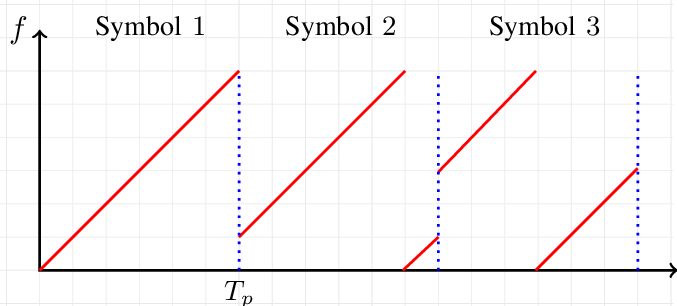
\includegraphics[scale=.4]{figures/asstes/n-LoRa-CSS-each-symbol-is-encoded-as-a-single-circularly-shifted-chirp-and-covers-the.png}
\caption{LoRa Symbole | Quelle: \cite{inproceedings}}
\label{fig:lora-symbole}
\end{figure}

\paragraph*{Erkennung unterhalb des Rauschpegels}
Die Fähigkeit, Signale unterhalb des Rauschpegels zu detektieren, basiert auf der \textit{Korrelation} zwischen empfangenem Signal und den orthogonalen Referenz-Chirps. Da LoRa-Symbole die gesamte Bandbreite $B$ abtasten, erfolgt eine Art \textit{Spektralspreizung}, die eine Energieintegration über die gesamte Symbolzeit ermöglicht. Der optimale Empfänger multipliziert das Empfangssignal mit einem Downchirp und führt anschließend eine diskrete Fourier-Transformation (DFT) durch. Das Maximum im Frequenzspektrum gibt den übertragenen Symbolindex an (siehe Formel \ref{eq:lorasymbolindex2}).
\begin{equation}
\label{eq:lorasymbolindex2}
\hat{s}(nT_s) = \arg \max_p \left| \sum_{k=0}^{2^{SF}-1} r(nT_s+kT) \cdot e^{-j 2\pi \frac{k^2}{2^{SF}}} \cdot e^{-j 2\pi \frac{p k}{2^{SF}}} \right|
\end{equation}
Durch die Integration über $T_s$ kann das Signal-Rausch-Verhältnis effektiv erhöht werden, wodurch eine Dekodierung auch unterhalb des thermischen Rauschpegels möglich ist. \autocite{tulkaLoRaSpreadingFactor, 8067462}


\subsubsection*{LoraWAN} 
\label{sec:lorawan}

LPWANs (Low Power Wide Area Networks) ermöglichen energieeffiziente Kommunikation über große Distanzen und gelten daher als eine Schlüsseltechnologie für das Internet der Dinge (IoT). LoRaWAN zählt zu den vielversprechendsten LPWAN-Technologien. Es bietet geringe Leistungsaufnahme, niedrige Kosten und große Reichweite, geht jedoch mit einer geringen Datenrate einher.

Das LoRaWAN-Kommunikationssystem besteht aus Endgeräten, Gateways, einem Netzwerkserver und den jeweiligen Anwendungen. Die Endgeräte kommunizieren über Funk mit den Gateways, welche die Daten an den Netzwerkserver weiterleiten. Von dort aus können dann andere Applikationen, meist über MQTT, die Daten auslesen und verwerten. 

\paragraph*{LoRaWAN-Geräteklassen}
Die LoRaWAN-Spezifikation definiert drei Endgeräteklassen \autocite{sornin2015lorawan}:

\begin{itemize}
    \item \textbf{Class A:} Für batteriebetriebene Geräte optimiert. Unterstützt bidirektionale Kommunikation mit einem Uplink-Fenster, gefolgt von zwei Downlink-Empfangsfenstern (RX1, RX2). Diese Funktionalität muss auf allen LoRaWAN-Geräten implementiert werden.
    
    \item \textbf{Class B:} Bietet zusätzlich geplante Empfangsfenster für vorhersagbare Downlinks. Geräte beginnen als Class A und können vom Server in Class B versetzt werden.
    
    \item \textbf{Class C:} Für netzbetriebene Geräte mit kontinuierlich offenem Empfangsfenster (RX2), was geringe Latenz ermöglicht. Diese Geräte verbrauchen mehr Energie im Vergleich zu anderen Geräteklassen.
\end{itemize}

\paragraph*{Leistungsmerkmale und Herausforderungen}
LoRaWAN kann durch Parameteroptimierung an unterschiedliche Anwendungen angepasst werden. Wichtige Designaspekte sind Skalierbarkeit, Durchsatz, Abdeckung, Energieeffizienz und geringe Kosten \cite{bor2017lora}. Herausforderungen bestehen insbesondere in:

\begin{itemize}
    \item \textbf{Skalierbarkeit:} Beeinflusst durch Faktoren wie verfügbare Kanäle, Spreizfaktor, Bandbreite und regulatorische Einschränkungen. In Europa steht für LoRa das Band von 863 MHz bis 870 MHz zur Verfügung, in Amerika von 902 MHz bis 928 MHz \autocite{FrequencyPlans}.
    
    \item \textbf{Energieeinsparung:} Durch die Adaptive Data Rate (ADR) oder eine optimierte Parameterwahl kann durch LoraWAN nochmals zusätzlich zu der ohnehin schon EStromspaarenden Lora-Technologie Energie eingespaart werden \autocite{kufakunesuSurveyAdaptiveData2020}.
    
    \item \textbf{Sicherheit:} Bei LoRaWAN spielt Sicherheit eine sehr wichtige Rolle, da Daten über Funk übertragen werden und damit leicht abgefangen werden könnten. Um das zu verhindern, werden Ende-zu-Ende-Schlüssel verwendet. Das bedeutet, dass Nachrichten bereits beim Gerät verschlüsselt werden und nur die dafür vorgesehenen Server diese wieder entschlüsseln können.  In der Praxis wird meist das Verfahren \emph{OTAA} (Over-The-Air Activation) eingesetzt. Dabei meldet sich das Gerät zunächst mit einem sogenannten Join-Vorgang am Netzwerk an. Hierfür gibt es einen eigenen \emph{Join Server}, der für die Schlüsselverwaltung zuständig ist. Nach erfolgreichem Join erhält das Gerät individuelle Sitzungsschlüssel, die für die eigentliche Kommunikation genutzt werden.  In öffentlichen Netzen ist es besonders wichtig, dass die verschiedenen Aufgaben klar voneinander getrennt sind. Der \emph{Join Server} übernimmt die Schlüsselverwaltung und den Beitritt, der \emph{Network Server} kümmert sich um die Organisation und Sicherheit des Funknetzes, und der \emph{Application Server} verarbeitet am Ende die entschlüsselten Anwendungsdaten. Diese Aufgabentrennung verhindert, dass Betreiber oder andere Parteien mehr Informationen einsehen können, als für sie notwendig ist. Außerdem wird dadurch eine sichere Verwaltung von Schlüsseln in Lieferketten und bei mehreren Nutzern (Multi-Tenant) ermöglicht, ohne dass ein Verlust der Schlüssel (\emph{Key Custody}) droht.  Damit die verschiedenen Server reibungslos zusammenarbeiten, wurden standardisierte Schnittstellen (Backend-Interfaces) entwickelt, die genau festlegen, wie die Kommunikation zwischen den Komponenten erfolgen soll. Untersuchungen zeigen zudem, dass die neuere Version \emph{LoRaWAN 1.1} deutliche Sicherheitsverbesserungen im Vergleich zur älteren Version 1.0 bietet. \autocite{butun2019security, LoRaWANBackendInterfaces11}

\end{itemize}

\paragraph*{Join-Mechanismus (OTAA)}
\label{sec:joinmechanissmus_otaa}
Bei der \emph{Over-The-Air Activation (OTAA)} meldet sich ein Endgerät bei dem Netzwerk an, indem es eine \emph{Join-Request}-Nachricht mit \emph{JoinEUI} (in LoRaWAN~1.0.x \emph{AppEUI}), \emph{DevEUI} und einem inkrementierenden \emph{DevNonce} sendet. Der \emph{DevNonce} ist ein 16-Bit-Wert und darf nie wiederverwendet werden. Dieser Wert muss in einem persistenten Speicher verwaltet werden. Der \emph{Join Server} prüft die Anfrage, generiert Sitzungsschlüssel und sendet eine verschlüsselte \emph{Join-Accept}-Nachricht zurück. In LoRaWAN~1.0.x werden dabei \emph{NwkSKey} und \emph{AppSKey} abgeleitet. In LoRaWAN~1.1 ersetzt ein erweitertes Schlüsselschema das \emph{NwkSKey} durch mehrere Netzwerkschlüssel (\emph{FNwkSIntKey}, \emph{SNwkSIntKey}, \emph{NwkSEncKey}). Der \emph{AppSKey} bleibt für Applikationsdaten bestehen. Eine erneute Anmeldung wird nur erforderlich, wenn Sitzungsschlüssel erneuert werden müssen. \autocite{thethingsnetworkJoin,techplayonJoin}

\paragraph*{Anwendungsgebiete}
LoRaWAN eignet sich für zahlreiche IoT-Szenarien, darunter smarte digitale Städte, smarte Messungen für zum Beispiel Pflanzen, smarter Parkverkehr indem Autofarern und Autofahrerinnen der weg zu einem freien Parkplatzt gezeigt wird oder intelligente Straßenbeleuchtung \autocite{BadenWuerttembergFoerdertLong2024}. Aufgrund der niedrigen Bitrate ist der Einsatz jedoch auf Anwendungen mit geringer Datenübertragungsrate beschränkt.

\paragraph*{Roaming, Peering und Interoperabilität}
LoRaWAN-Roaming erlaubt es, dass Endgeräte auch außerhalb des eigenen Netzwerks funktionieren können. Es gibt zwei Arten von Roaming:

\begin{itemize}
  \item \textbf{Passives Roaming:} Das Endgerät bleibt unter der Kontrolle seines Heimat-Netzservers (Serving NS), die Funkverbindung läuft aber über fremde Gateways und Netzserver (Forwarding NS). Diese leiten die Daten nur weiter, ohne die eigentliche Gerätesteuerung zu übernehmen.
  \item \textbf{Handover Roaming:} Hier übergibt der Heimat-Netzserver die Kontrolle an einen besuchten Netzserver (Serving NS). Dieser steuert dann das Endgerät aktiv, während der Heimat-NS im Hintergrund für die Schlüsselaushandlung und Verwaltung eingebunden bleibt.
\end{itemize}

Damit Roaming überhaupt funktioniert, müssen Netzbetreiber Peering- oder Roamingabkommen schließen. 
\emph{Packet Broker} bietet dazu ein globales Vermittlungsnetz, das den Austausch von Paketen zwischen verschiedenen Betreibern erleichtert. Ein Beispiel ist das offene Netz \texttt{The Things Network (TTN)} mit der \texttt{NetID~000013}. 

Kommerzielle Anbieter wie Senet setzen zusätzlich auf bilaterale Roaming-Vereinbarungen mit Partnernetzen, um ihre Abdeckung zu erweitern. \cite{LoRaWANBackendInterfaces11,PacketBroker,TTNNetID,SenetExt}


\paragraph*{Regulatorische Rahmenbedingungen (EU)}
In Europa wird das EU863–870-Band für LoRaWAN verwendet mit \emph{Duty-Cycle}-Grenzen je Subband (typisch 0{,}1–1\,\%\,/ 10\,\% im 869{,}4–869{,}65\,MHz-Subband) und Sendeleistungsgrenzen. Gerätekonfiguration und Kanalpläne folgen den \emph{LoRa Alliance Regional Parameters} (RP002), während die verbindlichen Funkparameter in \emph{ETSI EN~300~220} festgelegt sind. 
\autocite{RP002104, ETSIEN3002202025}